\documentclass[12pt]{article}
\usepackage{enumitem}
\usepackage[letterpaper,left=2cm,right=2cm,top=2cm,bottom=2cm]{geometry}
\usepackage{tikz-cd,amsmath,amssymb}
\usepackage{graphicx}
\newenvironment{QandA}
{
	\begin{enumerate}[label=\normalfont\arabic*.,leftmargin=2em,rightmargin=2em]\normalfont
	}
	{
	\end{enumerate}
}
\newenvironment{codelalala}{}{}
\newenvironment{answered}{\setlength{\parindent}{1em}\par\normalfont}{}
\usepackage{lipsum}
\pagestyle{empty}
\title{CSE 573 Fall 2018 Project 1}
\author{Pratik Pravin Kubal}
\date{UB Person Number: 50290804}
\pagestyle{plain}
\begin{document}
	\noindent%
	\maketitle
	\begin{QandA}
		\item Edge Dectection
		\\
			Write programs to detect edges in Fig. 1 (along both x and y directions) using Sobel operator. In your report, please include two resulting images, one showing edges along x direction and the other showing edges along y direction.
	\begin{answered}
		For Edge detection firstly I used the basic functions from cv library to read and write. While working on it, previously I had Normalized directly by taking the value 255 as the max value. However, later on I used absolute values method given in "demo.py". Both methods gave similar results.
		\\
		The Normalization used: 
		abs(image)/max(abs(image))
		\\
		Since I am using float array, I had problem writing the image, it was black because the values of pixels were very less, therefore, I multiplied the pixel values by 255 to get an image that I can write.
		\\
		\begin{figure}
		\centering
  			\fbox{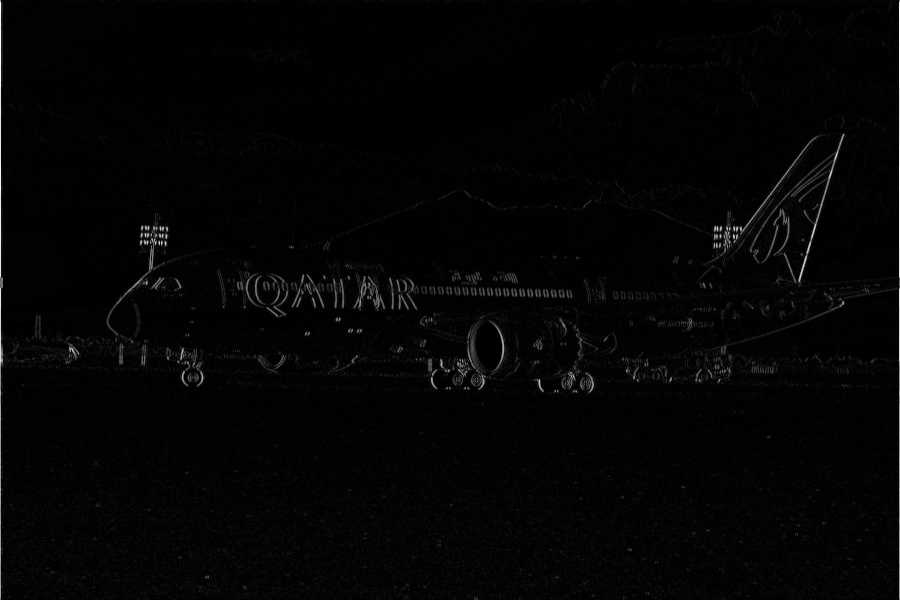
\includegraphics[scale=0.25]{./edge_x.jpg}
  					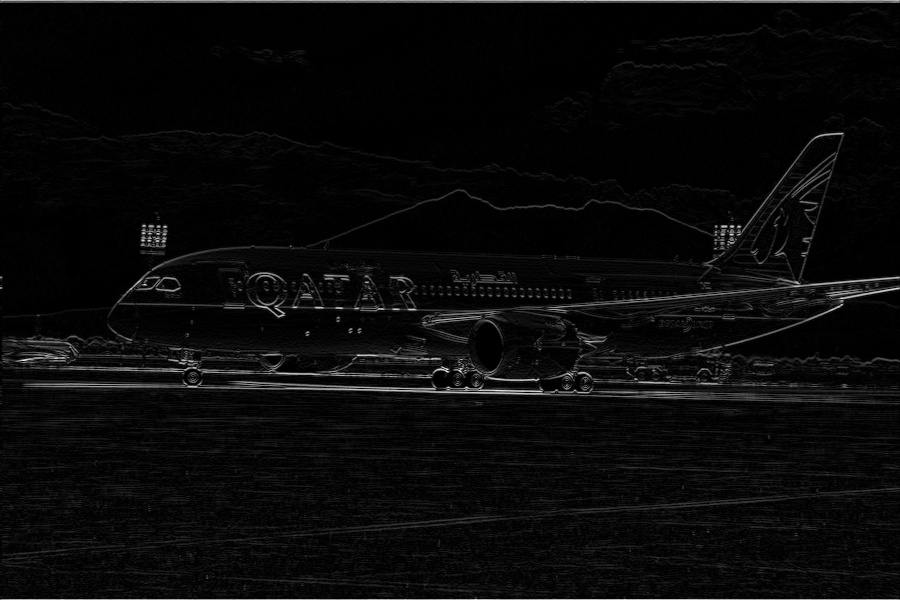
\includegraphics[scale=0.25]{./edge_y.jpg}}
  			\caption{Edge Detection along x axis and y axis }
  		\label{edge-detection}
\end{figure}
		For functions used to build Edge detection are as follows:
		\begin{codelalala}
		\begin{verbatim}
		def rgbToGrayscale(image):
    		r,g,b = image[:,:,0],image[:,:,1],image[:,:,2]
    		grayscaleImage =  0.299*r + 0.587*g + 0.114*b
    		return grayscaleImage
    	\end{verbatim}
		\begin{verbatim}
		def windowMult(matA,matB):
    		matResult = 0
    		for x_iter in range(0,getShape(matA)[0]):
        		for y_iter in range(0,getShape(matA)[0]):
            		if not len(matA) or not len(matB) == 0:
                		matResult += matA[x_iter][y_iter] * matB[x_iter][y_iter]
    		return matResult
		\end{verbatim}
		\begin{verbatim}
		def padMat(matA,sizeWindow):
    		space = (int)(sizeWindow/2)
    		skeleton=[[] for i in range(0,(getShape(matA)[0]+(space*2)))]
    		for window_h in range(0,getShape(matA)[0]+(space*2)):
        		for window_w in range(0,getShape(matA)[1]+(space*2)):
            		if(window_h >= 0 and window_h <= (space-1)) or 
            		(window_h >getShape(matA)[0]+(space-1) 
            		and window_h <= getShape(matA)[0]+((space*2)-1) ):
                		skeleton[window_h].append(0)
            		else:
                		if(window_w >= 0 and window_w <= (space-1)) or 
                		(window_w > getShape(matA)[1]+(space-1)
                	 	and window_w <= getShape(matA)[1]+((space*2)-1)):
                    		skeleton[window_h].append(0)
               			else:
                    		skeleton[window_h].append(matA[window_h-(3)][window_w-(3)])
    		return skeleton
		\end{verbatim}
		\begin{verbatim}
		def sliceMat(matrix,window_h_start,window_h_stop,window_w_start,window_w_stop):
    		retMat = matrix[window_h_start:window_h_stop]
    		holdWindow = []
    		for i in range(0,len(retMat)):
        		holdWindow.append(retMat[i][window_w_start:window_w_stop])
    		return holdWindow
		\end{verbatim}
		\begin{verbatim}
		def normImage(matA):
    		skeleton=[[] for i in range(0,getShape(matA)[0])]
    		maxValue = 0
    		absValue = 0
		    for window_h in range(0,getShape(matA)[0]):
		        for window_w in range(0,getShape(matA)[1]):
        		    absValue = abs(matA[window_h][window_w])
		            skeleton[window_h].append(absValue)     
        		    if(maxValue < absValue) : 
        		    	maxValue = absValue
			returnMat=[[] for i in range(0,getShape(matA)[0])]
		    for window_h in range(0,getShape(matA)[0]):
        		for window_w in range(0,getShape(matA)[1]):
            		returnMat[window_h].append(skeleton[window_h][window_w] / maxValue)
    		return returnMat
		\end{verbatim}
		\begin{verbatim}
		def getShape(matA):
    		height = len(matA)
    		width = len(matA[1])
    		for i in range(0,height):
        		if(len(matA[i]) != width):
            		return -i
        		else:
            		return (height,width)
		\end{verbatim}	
    	\begin{verbatim}
		def invertMat(matA):
    		skeleton=[[] for i in range(0,getShape(matA)[0])]
    		i = 0
    		for window_h in range(getShape(matA)[0]-1,-1,-1):
        		for window_w in range(getShape(matA)[1]-1,-1,-1):
            		skeleton[i].append(matA[window_h][window_w])
       			i += 1
    		return skeleton
		\end{verbatim}
		\begin{verbatim}
def combineEdges(matA,matB):
    from math import sqrt
    maxValue = 0
    skeleton = [[] for i in range(0,getShape(matA)[0])]
    for window_h in range(0,getShape(matA)[0]):
        for window_w in range(0,getShape(matA)[1]):
            skeleton[window_h].append(sqrt(matA[window_h][window_w]**2 + matB[window_h][window_w]**2))
    for window_h in range(0,getShape(skeleton)[0]):
        for window_w in range(0,getShape(skeleton)[1]):
            if(skeleton[window_h][window_w]>maxValue): maxValue = skeleton[window_h][window_w]
    for window_h in range(0,getShape(skeleton)[0]):
        for window_w in range(0,getShape(skeleton)[1]):
            skeleton[window_h][window_w] = skeleton[window_h][window_w]/maxValue
    return skeleton
\end{verbatim}
		For actual sobel operator convolution I have used the following functions:
		\begin{verbatim}
		def sobel(matA,sobel_op):
    		matA = padMat(matA,3)
    		resultImage = [[]for i in range(600)]
    		for window_h in range(0,getShape(matA)[0]-2):
        		for window_w in range(0,getShape(matA)[1]-2):
            		window = sliceMat(matA,window_h,window_h+3,window_w,window_w+3)
            		opResult = windowMult(sobel_op,window)
            		resultImage[window_h].append(opResult)
    		resultImage = normImage(resultImage)
    		return resultImage
		\end{verbatim}
		The whole code which depends on these above functions is:
		\begin{verbatim}
from functions import rgbToGrayscale,windowMult,padMat,sliceMat,
normImage,getShape,invertMat,combineEdges,sobel
import numpy as np
import cv2

# Reading the Image
a = cv2.imread("./proj1_cse573/task1.png")
b = rgbToGrayscale(a)

# Define Operators
sobel_op_x = [[1,0,-1],
              [2,0,-2],
              [1,0,-1]]
sobel_op_y = [[-1,-2,-1],
              [0,0,0],
              [1,2,1]]

# Sobel Edges in x
edge_x = sobel(b,invertMat(sobel_op_x))

# Converting the image to display and write using cv libraries
edge_x_norm = np.asarray(edge_x)
edge_x_norm = edge_x_norm * 255
edge_x_norm = edge_x_norm.astype('uint8')
cv2.imwrite("edge_x.jpg",edge_x_norm)

# Sobel Edges in x
edge_y = sobel(b,invertMat(sobel_op_y))


# Converting the image to display and write using cv libraries
edge_y_norm = np.asarray(edge_y)
edge_y_norm = edge_y_norm * 255
edge_y_norm = edge_y_norm.astype('uint8')
cv2.imwrite("edge_y.jpg",edge_y_norm)

# Combining edge detection in x and y
combined = combineEdges(edge_x,edge_y)
combined_norm = np.asarray(combined)
combined_norm = combined_norm * 255
combined_norm = combined_norm.astype('uint8')
cv2.imwrite("combined.jpg",combined_norm)

print("Original image size: {:4d} x {:4d}".format(a.shape[0], a.shape[1]))
print("Resulting image size: {:4d} x {:4d}".format(combined_norm.shape[0], combined_norm.shape[1]))
		\end{verbatim}
		\end{codelalala}
		Observations:
        \\
        Edge detection along x and y directions have been computed(See Fig \ref{edge-detection}). I have also combined both the edges, see Fig. \ref{edge-detection-combined}. When I was using the old basic divide by 255 normalizations, I was missing few edges, however, when I used the absolute-valued normalization, the results were better.
	\begin{figure}
		\centering
  			\fbox{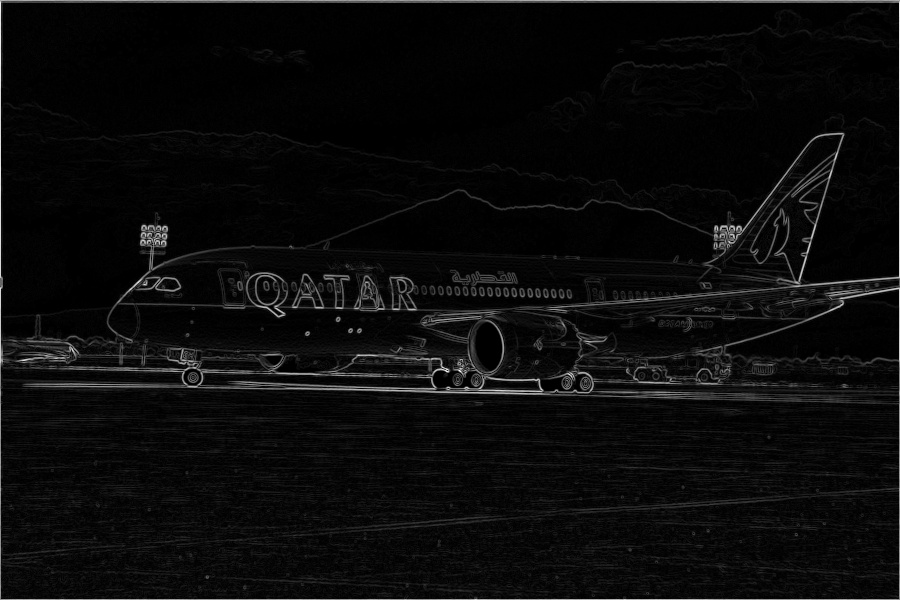
\includegraphics[scale=0.25]{./combined.jpg}}
  			\caption{Combined edge detected in x and y axis}
  		\label{edge-detection-combined}
	\end{figure}
	\end{answered}
	\item Keypoint Detection
	\\
	\\
	Write programs to detect keypoints in an image according to the following steps, which are also the first three steps of Scale-Invariant Feature Transform (SIFT).
\begin{answered}
I am using the method discussed by the TA and used by openCV of multiplying with the constant to generate Gaussian Kernel. The formula for it is as follows:
\\
C = $\frac{1}{\sum_{i=-2}^{2}\sum_{j=-2}^{2}f(i,j)}$
\\
Where, f(i,j) is the gaussian function
\\
The functions used for this task is as follows:
\begin{codelalala}
\begin{verbatim}
def genOctave(matA):
    skeleton = [[] for i in range(0,(int)(getShape(matA)[0]/2))]
    for window_h in range(0,getShape(matA)[0]):
        for window_w in range(0,getShape(matA)[1]):
            if(window_h % 2 ==0 and window_w % 2 == 0):
                sampleIndex = (int)(window_h / 2)
                if(sampleIndex < (int)(getShape(matA)[0]/2)):
                    skeleton[sampleIndex].append(matA[window_h][window_w])
    return(skeleton)
\end{verbatim}
\begin{verbatim}
def genGaussianVal(xval,yval,sigma):
    import math
    sigma = sigma**2
    return (1/(2*math.pi*sigma))*math.exp(-((xval**2+yval**2)/(2*sigma)))
\end{verbatim}
\begin{verbatim}
def summession2d(matA):
    summession = 0
    for window_h in range(0,getShape(matA)[0]):
        for window_w in range(0,getShape(matA)[1]):
            summession += matA[window_h][window_w]
    return summession
\end{verbatim}
\begin{verbatim}
def genGaussianKernel(scales,octaveNumber,scalesNumber):
    from functions import genGaussianVal,summession2d
    gaussianKernel = [[] for i in range(0,7)]
    scalesStack = scales[octaveNumber-1]
    sigma = scalesStack[scalesNumber-1]
    i = 0
    for y in range(3,-4,-1):
        for x in range(-3,4,1):
            gaussianKernel[i].append(genGaussianVal(x,y,sigma))
        i+=1
    constant = summession2d(gaussianKernel)
    constant = 1/constant
    for y in range(0,7):
        for x in range(0,7):
            gaussianKernel[y][x] = constant*gaussianKernel[y][x] 
    return gaussianKernel
\end{verbatim}
\begin{verbatim}
def convolve(windowFilter,matA):
    from functions import invertMat,getShape,sliceMat,padMat,windowMult
    windowFilter = invertMat(windowFilter)
    matA = padMat(matA,getShape(windowFilter)[0])
    resultImage = [[] for i in range(0,(getShape(matA)[0] - 
    (getShape(windowFilter)[0] - 1)))]
    for window_h in range(0,getShape(matA)[0]-
    (getShape(windowFilter)[0] - 1)):
        for window_w in range(0,getShape(matA)[1]-
        (getShape(windowFilter)[1] - 1) ):
            window = sliceMat(matA,window_h,window_h+
            getShape(windowFilter)[0],window_w,window_w +getShape(windowFilter)[0])
            opResult = windowMult(windowFilter,window)
            resultImage[window_h].append(opResult)
    return resultImage
\end{verbatim}
\begin{verbatim}
def differenceGaussians(matA,matB):
    if(getShape(matA) == getShape(matB)):
        skeleton = [[] for i in range(0,getShape(matA)[0])]
        for window_h in range(0,getShape(matA)[0]):
            for window_w in range(0,getShape(matB)[1]):
                difference = matA[window_h][window_w] - matB[window_h][window_w] 
                skeleton[window_h].append(difference)
        return skeleton
    else:
        return -1
\end{verbatim}
\begin{verbatim}
def isMinima(dogslice,center,isMid):
    counter=0
    if(not isMid):
        for window_h in range(0,3):
            for window_w in range(0,3):
                if dogslice[window_h][window_w] > center:
                    counter +=1
        if(counter == 9):
            return True
        else:
            return False
    else:
        for window_h in range(0,3):
            for window_w in range(0,3):
                if(window_h != 1 or window_w != 1):
                    if (dogslice[window_h][window_w] > center):
                        counter +=1
        if(counter == 8):
            return True
        else:
            return False
\end{verbatim}
\begin{verbatim}
def isMaxima(dogslice,center,isMid):
    counter = 0
    if(not isMid):
        for window_h in range(0,3):
            for window_w in range(0,3):
                if dogslice[window_h][window_w] < center:
                    counter += 1
        if(counter == 9):
            return True
        else:
            return False
    else:
        for window_h in range(0,3):
            for window_w in range(0,3):
                if window_h != 1 or window_w != 1 :
                    val = dogslice[window_h][window_w]
                    if val < center:
                        counter +=1
        if(counter == 8):
            return True
        else:
            return False
\end{verbatim}
\begin{verbatim}
def findMinimaMaxima(dogstack,mainImage,octaveNumber,tracker):
    for mid_window_h in range(0,(getShape(dogstack[1])[0] - 2)):
        for mid_window_w in range(0,(getShape(dogstack[1])[1] - 2)):
            middogslice = sliceMat(dogstack[1],mid_window_h,(mid_window_h+3),
            mid_window_w,mid_window_w+3)
            upperdogslice = sliceMat(dogstack[0],mid_window_h,(mid_window_h+3),
            mid_window_w,mid_window_w+3)
            lowerdogslice = sliceMat(dogstack[2],mid_window_h,(mid_window_h+3),
            mid_window_w,mid_window_w+3)
            center = middogslice[1][1]
            h_coords = mid_window_h+1
            w_coords = mid_window_w+1
            if(getShape(upperdogslice)[0] == 3 and getShape(upperdogslice)[1] == 3):
                if(isMinima(middogslice,center,True) 
                and isMinima(upperdogslice,center,False) 
                and isMinima(lowerdogslice,center,False)):
                    print("Keypoint Minima!");
                    print(mid_window_h,mid_window_w)
                    mainImage[h_coords*octaveNumber][w_coords*octaveNumber] = 255
                    count+=1
                    tracker.append([h_coords*octaveNumber,w_coords*octaveNumber])
                elif(isMaxima(middogslice,center,True)
                 and isMaxima(upperdogslice,center,False)
                  and isMaxima(lowerdogslice,center,False)):
                    print("Keypoint Maxima!");
                    print(mid_window_h,mid_window_w)
                    mainImage[h_coords*octaveNumber][w_coords*octaveNumber] = 255
                    count+=1
                    tracker.append([h_coords*octaveNumber,w_coords*octaveNumber])             
    return mainImage
\end{verbatim}
\begin{verbatim}
def ecl_distance(tracker):
    import math
    [x,y] = tracker
    return math.sqrt((y-0)**2+(x-0)**2)
\end{verbatim}
The Main Program for finding keypoints
\begin{verbatim}
from functions import rgbToGrayscale,genOctave,convolve,genGaussianKernel,
differenceGaussians,findMinimaMaxima,ecl_distance
import cv2
import numpy as np

a = cv2.imread("./proj1_cse573/task2.jpg")
b = rgbToGrayscale(a)

scales=[[0.70710678118,1,1.41421356237,2,2.82842712475],
        [1.41421356237,2,2.82842712475,4,5.65685424949],
        [2.82842712475,4,5.65685424949,8,11.313708499],
        [5.65685424949,8,11.313708499,16,22.627416998]]

# genGaussianKernel(scales,octaveNumber,scalesNumber)
octave1 = b.copy()
windowFilter = genGaussianKernel(scales,1,1)
octave1_1 = convolve(windowFilter,octave1)
octave1_1_norm = np.asarray(octave1_1)
cv2.imwrite("octave1_1_norm.jpg",octave1_1_norm)

----- For Each Octave -----

# Difference of Gaussians
# 2nd arg - 1st arg
dog1_1 = differenceGaussians(octave1_1,octave1_2)
dog1_1_norm = np.asarray(dog1_1)
cv2.imwrite("dog1_1_norm.jpg",dog1_1_norm)

----- For Each Difference of Gaussians -----

# Key Points detection
outputImage = a.copy()
stack1_1 = [dog1_1,dog1_2,dog1_3]
keypointsMat1_1 = findMinimaMaxima(stack1_1,outputImage,1,tracker)
stack1_2 = [dog1_2,dog1_3,dog1_4]
keypointsMat1_2 = findMinimaMaxima(stack1_2,outputImage,1,tracker)

----- For Each Keypoint Detection -----

cv2.imwrite("keypoints.jpg",outputImage)
ecl_distance_sort = sorted(tracker,key=ecl_distance)
print("Closest five points are:")
print("Format is (Height,Width) or (y,x)")
print(ecl_distance_sort[0:5])
\end{verbatim}
\end{codelalala}
Each octave is half the previous one, therefore, the function of "genOctave" generates octaves while genGaussianKernel function generates the kernels. And {\ref{2nd-3rd-oct}} is what the question is asking. The resolution of the second octave is 375 by 229 pixels while that of the third octave is 118 by 114 pixels. 
\\
\begin{figure}
		\centering
  			\fbox{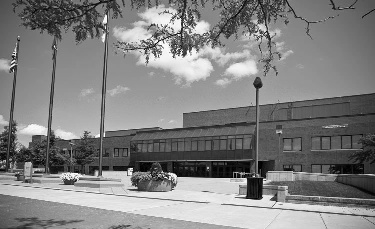
\includegraphics[scale=0.8]{./octave2_norm.jpg}
  			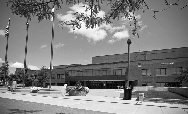
\includegraphics[scale=0.8]{./octave3_norm.jpg}}
  			\caption{Second and Third Octave}
  		\label{2nd-3rd-oct}
\end{figure}
The DoG images obtainted using the second and third octave are in fig:{\ref{2nd-3rd-dog} and \ref{2nd-3rd-dog-norm}}
\begin{figure}
		\centering
  			\fbox{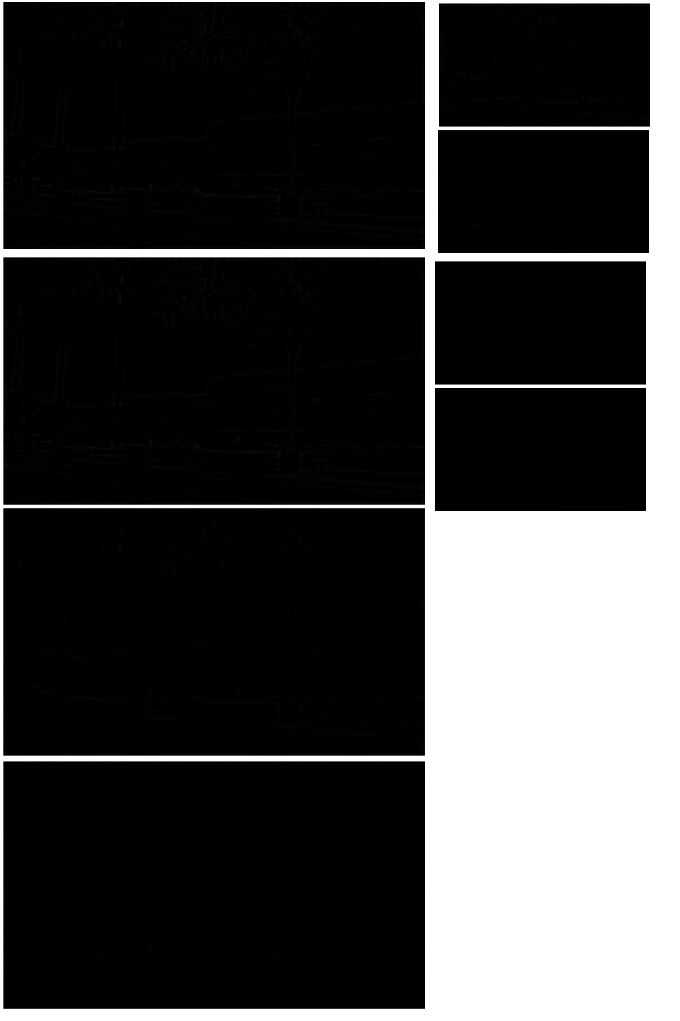
\includegraphics[scale=0.9]{./dog_pyrmd.png}}
  			\caption{The difference of Gaussian Pyramid}
  		\label{2nd-3rd-dog}
\end{figure}
\begin{figure}
		\centering
  			\fbox{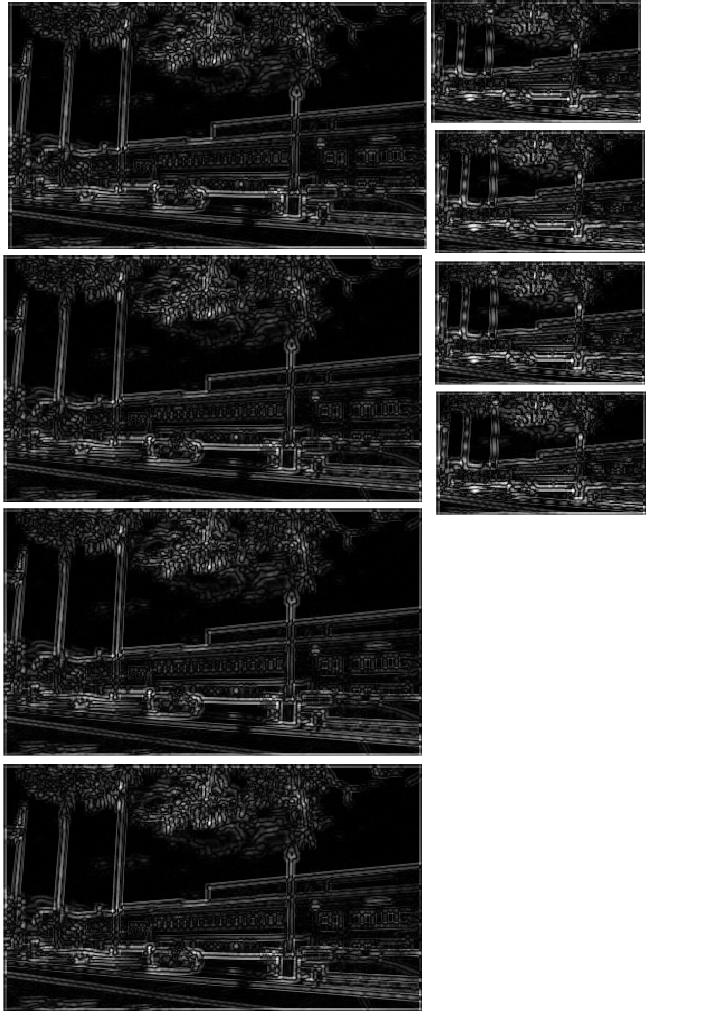
\includegraphics[scale=0.9]{./norm_dog.png}}
  			\caption{Normalized Gaussian Pyramid}
  		\label{2nd-3rd-dog-norm}
\end{figure}
\\
We perform first three steps of keypoint detection and plot the results back on the input image, see Fig{\ref{keypoint-result}}
\begin{figure}
		\centering
  			\fbox{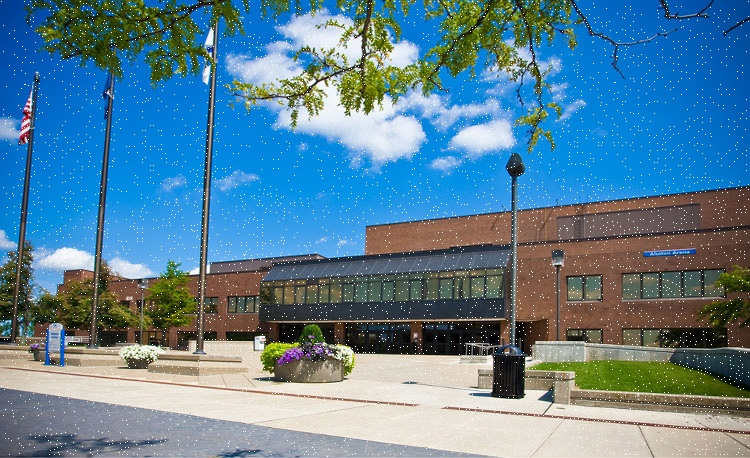
\includegraphics[scale=0.7]{./keypoints.jpg}}
  			\caption{Detected Keypoints on Original Image}
  		\label{keypoint-result}
\end{figure}
I think there are too many key points detected which are not relevant, I can see that in the top right corner, the key points are arranged perfectly on the branch, However, during areas of flat regions such as sky where every point is either minimal or maxima we are having problems. Also, we haven't found subpixel key points. After doing these steps we could get a better result.
\\
The coordinates of the five left-most detected key points are(Format is (Height, Width) or (y,x)):
\\
(1,1),(1,24),(25,3),(4,28),(1,30)
\\
\\
Footnote:
\\
\\
I tried detecting the key points as well as I could. But I think that my convolution function is not quite right. I know the concept of keypoints detection and convolution, however, I was unable to implement it properly.
\end{answered}
		\item For the task of cursor detection, which aims to locate the cursor in an image, two sets of images and cursor templates, named as ”Set A” and ”Set B”, will be provided to you. Set A is composed of a total number of 25 images and 1 cursor template. Set A is for task 1., i.e., the basic cursor detection which contributes to 5 points. Set B is composed of a total number of 30 images and 3 different cursor template. Set B is for task 2.,
\begin{answered}
Method:
\\
\\
In the start I have had tested my previous code of keypoint detection on this problem, however, I couldn't get good results. I also tried on pulling cv2.SIFT from GitHub repository(SIFT in OpenCV 3 is contrib package due to patent rights). This process made me realize that the Difference of Gaussians works better with template matching. Therefore, we need edges and template matching performs better with edges. This also made me understand the difference between Template matching and feature based methods. The main peculiarity of features is that during feature-based matching we have to match features which might be skewed. However, in this task, the cursor is free from translation invariance. Moreover, after looking at the dataset, it seems that we need to scale invariance.
\\
\begin{figure}
		\centering
  			\fbox{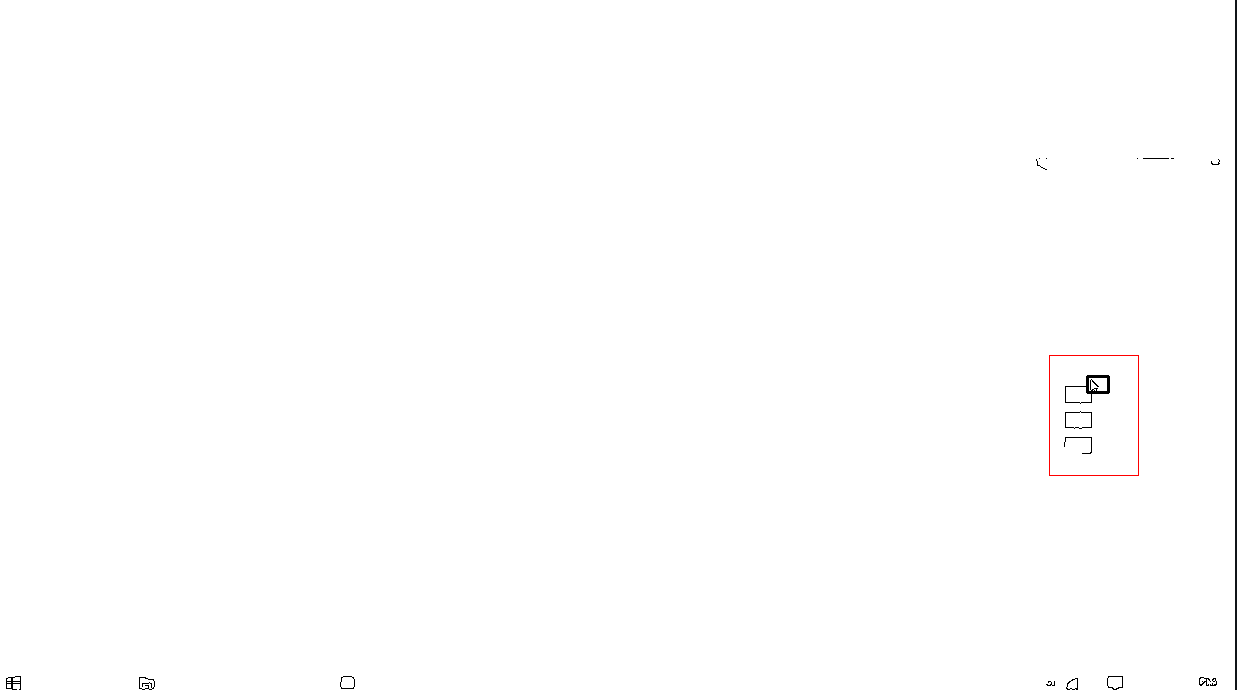
\includegraphics[scale=0.30]{./Cannyafter3scalings.png}}
  			\caption{pos$\_$3.jpg Using Canny after 3 downscalings (Inveted Image)}
  		\label{wow-canny-wow}
\end{figure}
\begin{figure}
		\centering
  			\fbox{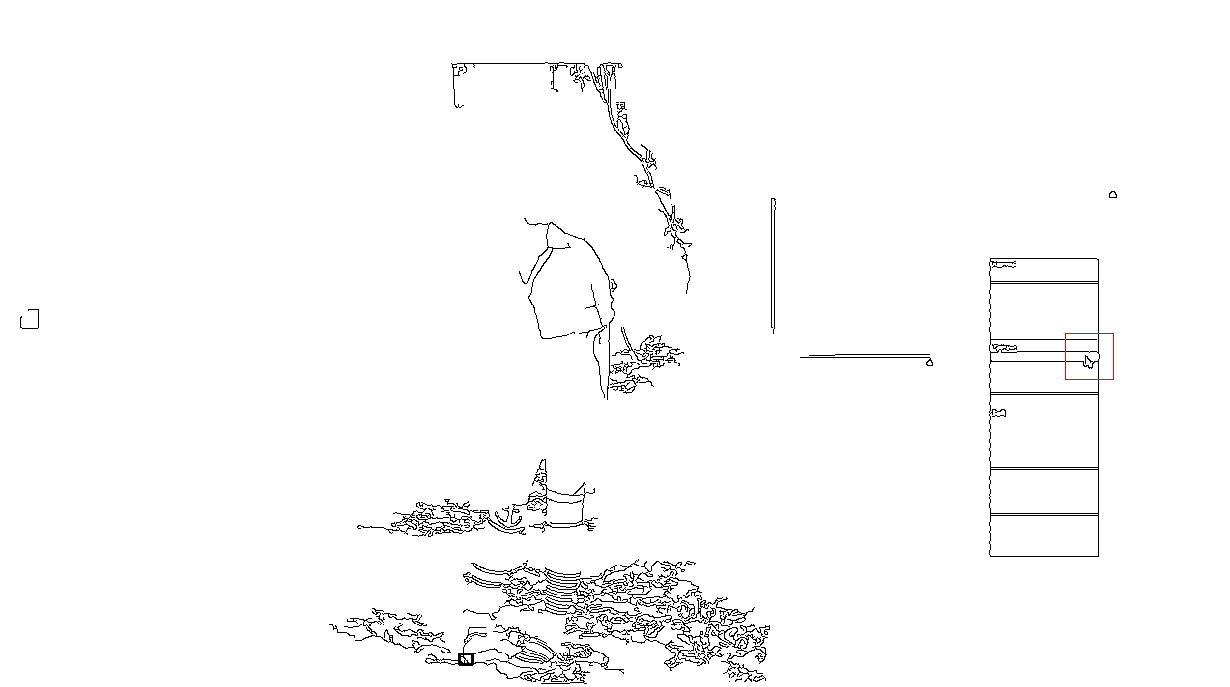
\includegraphics[scale=0.30]{./canyUnableToDetectcursor.png}}
  			\caption{pos$\_$9.jpg Red box shows that canny is unable to detect the cursor(Inveted Image)}
  		\label{canny-problem}
\end{figure}
For scale invariance, we are going to use what the Professor discussed about image stacks and resizing. We have two options to either resize the image or resize the template. However, if we sample the image and resize it could happen that we might lose information.
\\
After comparing the performance of Laplacian and Canny on the given template, I hypothesize that the result of canny would be better when the pointer is behind a different range of background due to the cursor wrapped in one-pixel boundary; See Fig.{\ref{wow-canny-wow}}. However, Canny is an edge detector, for an object like pointer it fails to detect it in some cases. See Fig.{\ref{canny-problem}}
\\
Therefore, I am taking the Gaussian-based approach for cursor detection.
\begin{figure}
		\centering
  			\fbox{
\includegraphics[scale=1]{./template_basic.png}}
  			\caption{Basic Cursor Detection Template}
  		\label{basic-template}
\end{figure}
1. Basic Cursor Detection
\\
I am using the cursor template given in Fig{\ref{basic-template}} and using the TM$\_$CCOEFF$\_$NORMED method of opencv.
\\
For basic Cursor Detection firstly I tried running it without any downscaling or upscaling of the template. There was a 20$\%$ accuracy on these methods. After using downscaling and upscaling of templates in my program, I was able to boost my accuracy and detect almost all the points in the basic Cursors. The accuracy as on writing this reports stands on not detecting any of negative images 10/10 and detecting 78.57$\%$ of positive pointers, which is 11 out of 14. Only 3 pointers were not detected. See {\ref{wow-basic-wow} and \ref{why-basic-why} } I am using a threshold of 0.6 to detect the pointers.
\begin{figure}
		\centering
  			\fbox{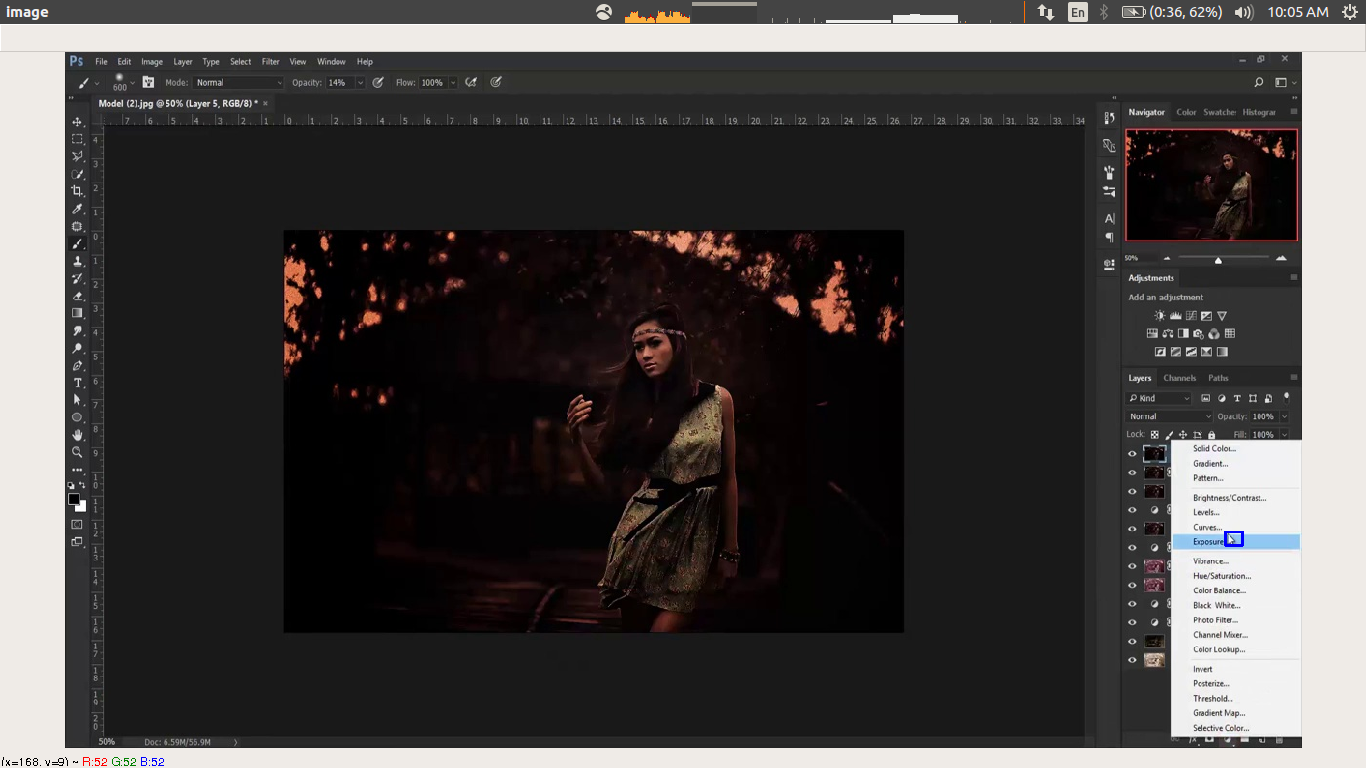
\includegraphics[scale=0.30]{./basic_cur_det.png}}
  			\caption{An example of good detection of cursor}
  		\label{wow-basic-wow}
\end{figure}
\begin{figure}
		\centering
  			\fbox{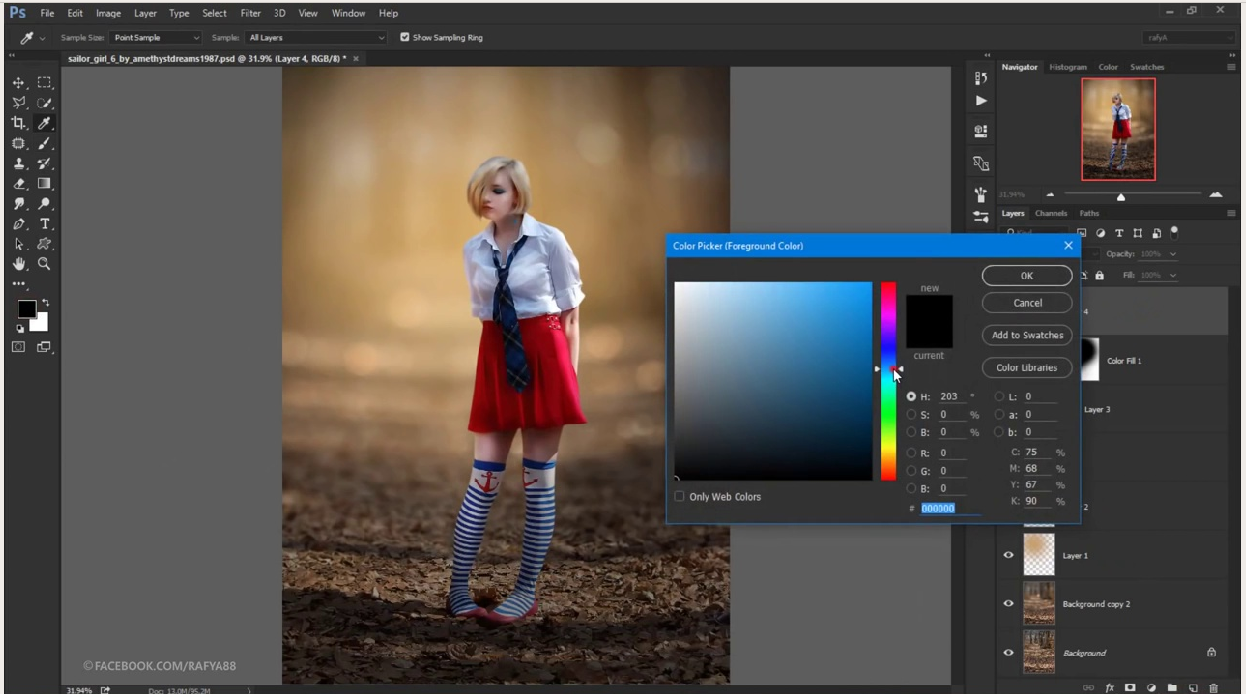
\includegraphics[scale=0.30]{./basic_cur_det_bad_case.png}}
  			\caption{Template Detection Failed to Detect any cursor}
  		\label{why-basic-why}
\end{figure}
2. Bonus Cursor Detection
\begin{figure}
		\centering
  			\fbox{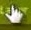
\includegraphics[scale=1]{./t1.jpg}}
  			\caption{Template for first set in bonus images}
  		\label{bonus1-template}
\end{figure}
The "t2" images so far give the best results, I was able to detect all the cursors from the images. However, the worst performance I got was by "t1" images, see
\begin{figure}
		\centering
  			\fbox{
\includegraphics[scale=1]{./t2.jpg}}
  			\caption{Template for second set in bonus images}
  		\label{bonus2-template}
\end{figure}
The third set of images "t3" also gives 100$\%$ accuracy, however, The bounding box is a bit small for some of the images, according to my program, the linspace starts with 1 and then decreases, which means this is a pure noise based match and for a large set of images it could suffer from salt and pepper noise, like we see in Fig{\ref{hand-cur-bad}}.
\begin{figure}
		\centering
  			\fbox{
\includegraphics[scale=1]{./t3_v2.jpg}}
  			\caption{Template for third set in bonus images}
  		\label{bonus3-template}
\end{figure}
The templates used for Bonus part are given in Fig\ref{bonus1-template},\ref{bonus2-template},\ref{bonus3-template}
\begin{figure}
		\centering
  			\fbox{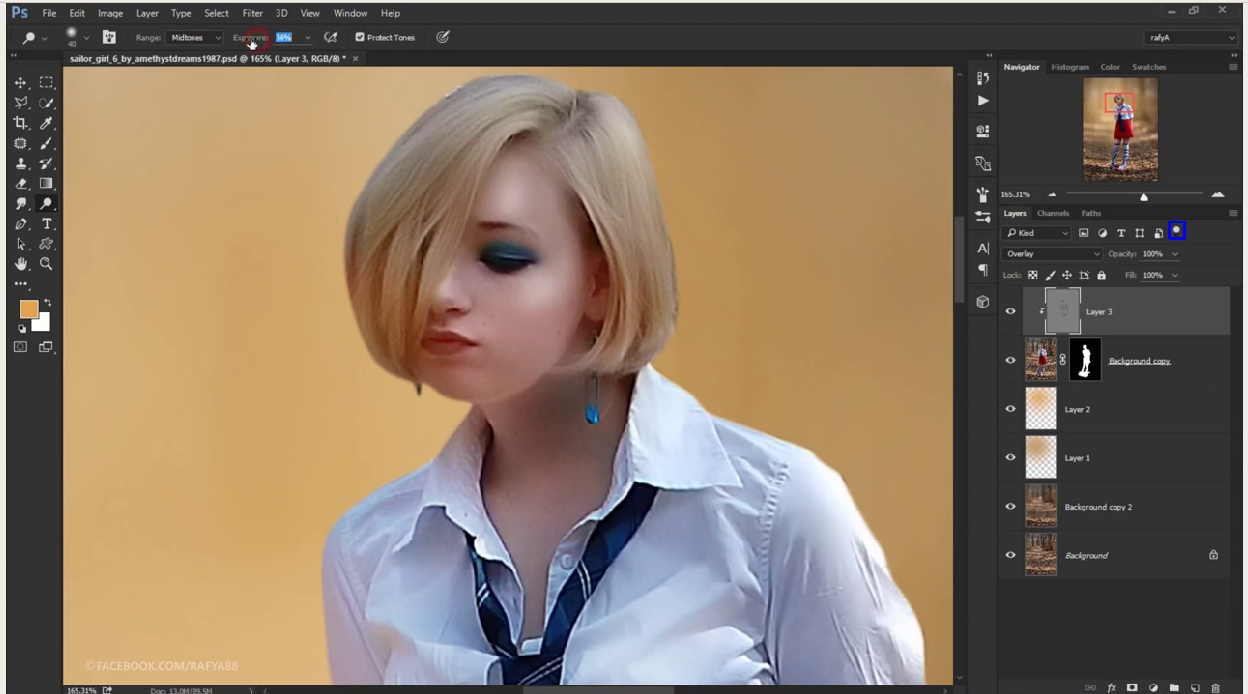
\includegraphics[scale=0.30]{./hand_cursor_worst_perf.jpg}}
  			\caption{Example of hand cursor bad performance}
  		\label{hand-cur-bad}
\end{figure}
Observations:
Let's talk about the worst performance of some of the detections which I had. Firstly, the hand cursor one seems like when I apply the Gaussian the hand cursor is practically indistinguishable from the knob-like button which photoshop has.
\\
Furthermore, template matching is also prone to problems such as a patch over the image area where the template is located might affect its performance. 
\\
The functions used are:
\begin{codelalala}
\begin{verbatim}
def matchTemplate(grayscaleImage,template):
    import cv2,imutils,numpy as np
    gaussianImage = cv2.GaussianBlur(grayscaleImage,(3,3),0)
    lap = cv2.Laplacian(gaussianImage,ddepth=32,ksize = 3)
    lapTemplate = cv2.Laplacian(template,ddepth=32,ksize=3)
    maxValFound = 0
    (storex,storey) = (0,0)
    (xcords,ycords) = (0,0)
    for downscale in np.linspace(1,0.5,20):
        if(int(lapTemplate.shape[1]*downscale) > 1):
            downscaledTemplate = imutils.resize(lapTemplate,
            int(lapTemplate.shape[1]*downscale))        
            a = cv2.matchTemplate(lap,downscaledTemplate,cv2.TM_CCOEFF_NORMED)
            (_,maxVal,_,(xval,yval)) = cv2.minMaxLoc(a)
            if maxVal > maxValFound:
                maxValFound = maxVal
                templateShape = np.shape(downscaledTemplate)
                (storexp,storeyp) =  (storex,storey)
                (storex,storey) = (xcords,ycords)
                (xcords,ycords) = (xval,yval)
    for upscale in np.linspace(2,1.02,20):
        if(int(lapTemplate.shape[1]*upscale) > 1):
            upscaledTemplate = imutils.resize(lapTemplate,
            int(lapTemplate.shape[1]*upscale))
            a = cv2.matchTemplate(lap,upscaledTemplate,cv2.TM_CCOEFF_NORMED)
            (_,maxVal,_,(xval,yval)) = cv2.minMaxLoc(a)
            if maxVal > maxValFound:
                maxValFound = maxVal
                templateShape = np.shape(downscaledTemplate)
                (storexp,storeyp) =  (storex,storey)
                (storex,storey) = (xcords,ycords)
                (xcords,ycords) = (xval,yval)
    return [maxValFound,templateShape,(xcords,ycords)]
\end{verbatim}
\end{codelalala}
\end{answered}
\end{QandA}
\end{document}